\documentclass[a4paper,11pt]{ltjsarticle}
\usepackage[margin=25mm]{geometry}
\usepackage{amsmath,amssymb}
\usepackage{graphicx}
\usepackage{float}

\title{工学実験 第三回課題}
\author{202025093 安川蒼真}
\date{2026/10/15}

\begin{document}
\maketitle

\section*{課題3.1}
Q学習がどのように進んでいるか，ディスプレイに描画されるエージェントの動きを図\ref{fig:photo1}に添付する．
\begin{figure}[H]
  \centering
  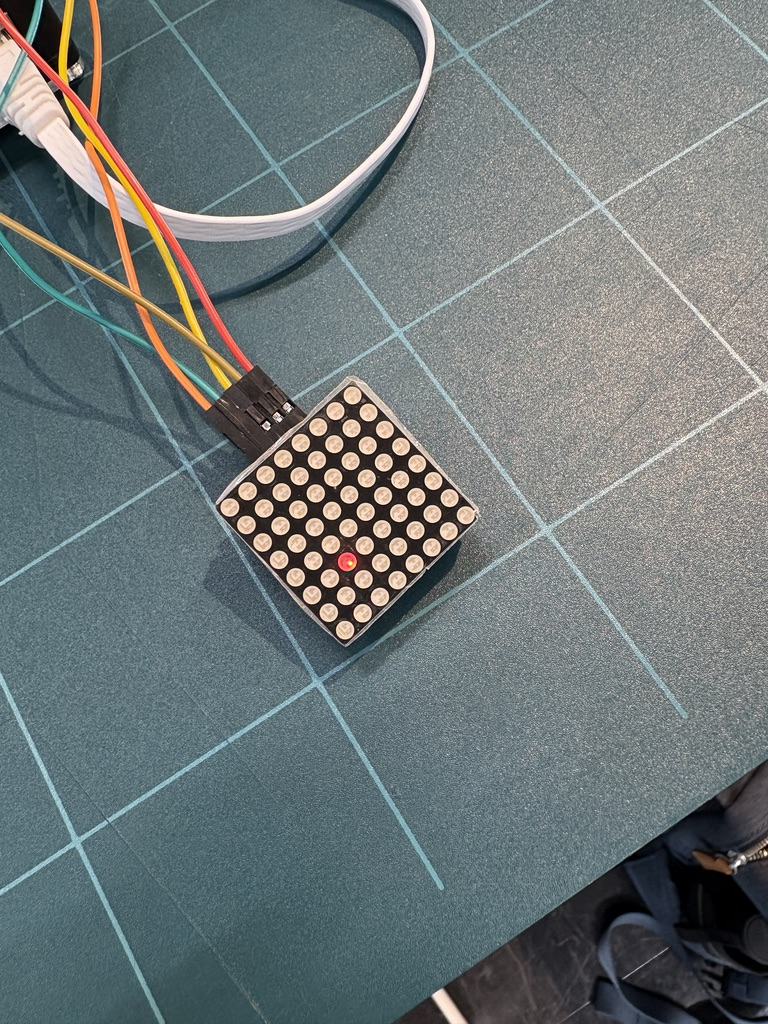
\includegraphics[width=0.3\linewidth]{photos/photo_1.jpeg}
  \caption{Q学習におけるエージェントの動作}
  \label{fig:photo1}
\end{figure}
学習初期には，エージェントが遠回りや同じ場所への移動を
繰り返す様子が見られた．
試行を重ねるにつれて，そのような動作が減少し，
より短い経路でゴールに到達する様子が確認できた．
\clearpage
\section*{課題3.2}
課題3.2および課題3.3では，提供されたプログラムのLED表示と待機処理を省き，
PC上でQ学習を再実行した．開始状態を9とし，ゴールを54および50として，
それぞれ1000回の試行を行った．学習率は0.1，割引率は0.9，探索率は0.3，
ゴール到達時の報酬は100とした．乱数シードは20261022とした．
以下のグラフ，Qテーブル，Q値マップは，各条件について同じ実行から取得したものである．

ステップ数の変化を図\ref{fig:steps54}，図\ref{fig:steps50}に示す．
横軸は試行番号（0から999），縦軸は1回の試行における実際の移動回数である．
元プログラムの出力ではゴールに入る最後の1歩が数えられないため，
本グラフではその1歩を含めて記録した．両条件とも1000回すべてでゴールに到達した．

\begin{figure}[H]
\centering
\begin{minipage}[t]{0.49\linewidth}
\centering
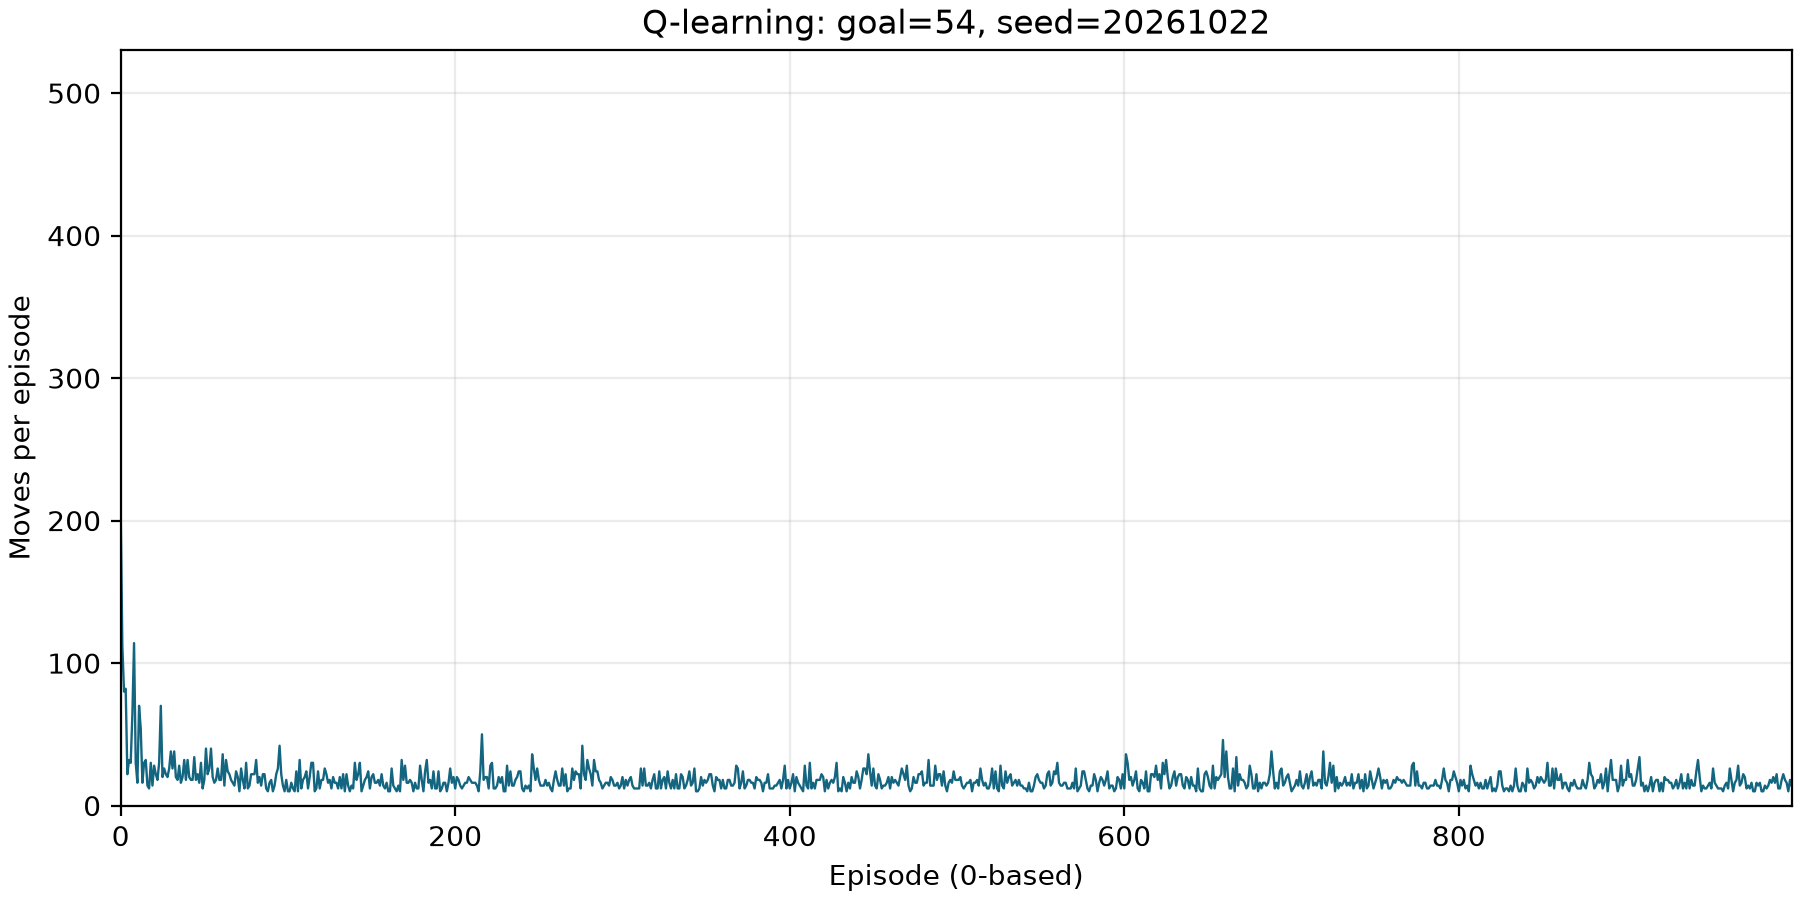
\includegraphics[width=\linewidth]{pc_results/terminal_54/steps.png}
\caption{ゴール54でのステップ数変化}
\label{fig:steps54}
\end{minipage}\hfill
\begin{minipage}[t]{0.49\linewidth}
\centering
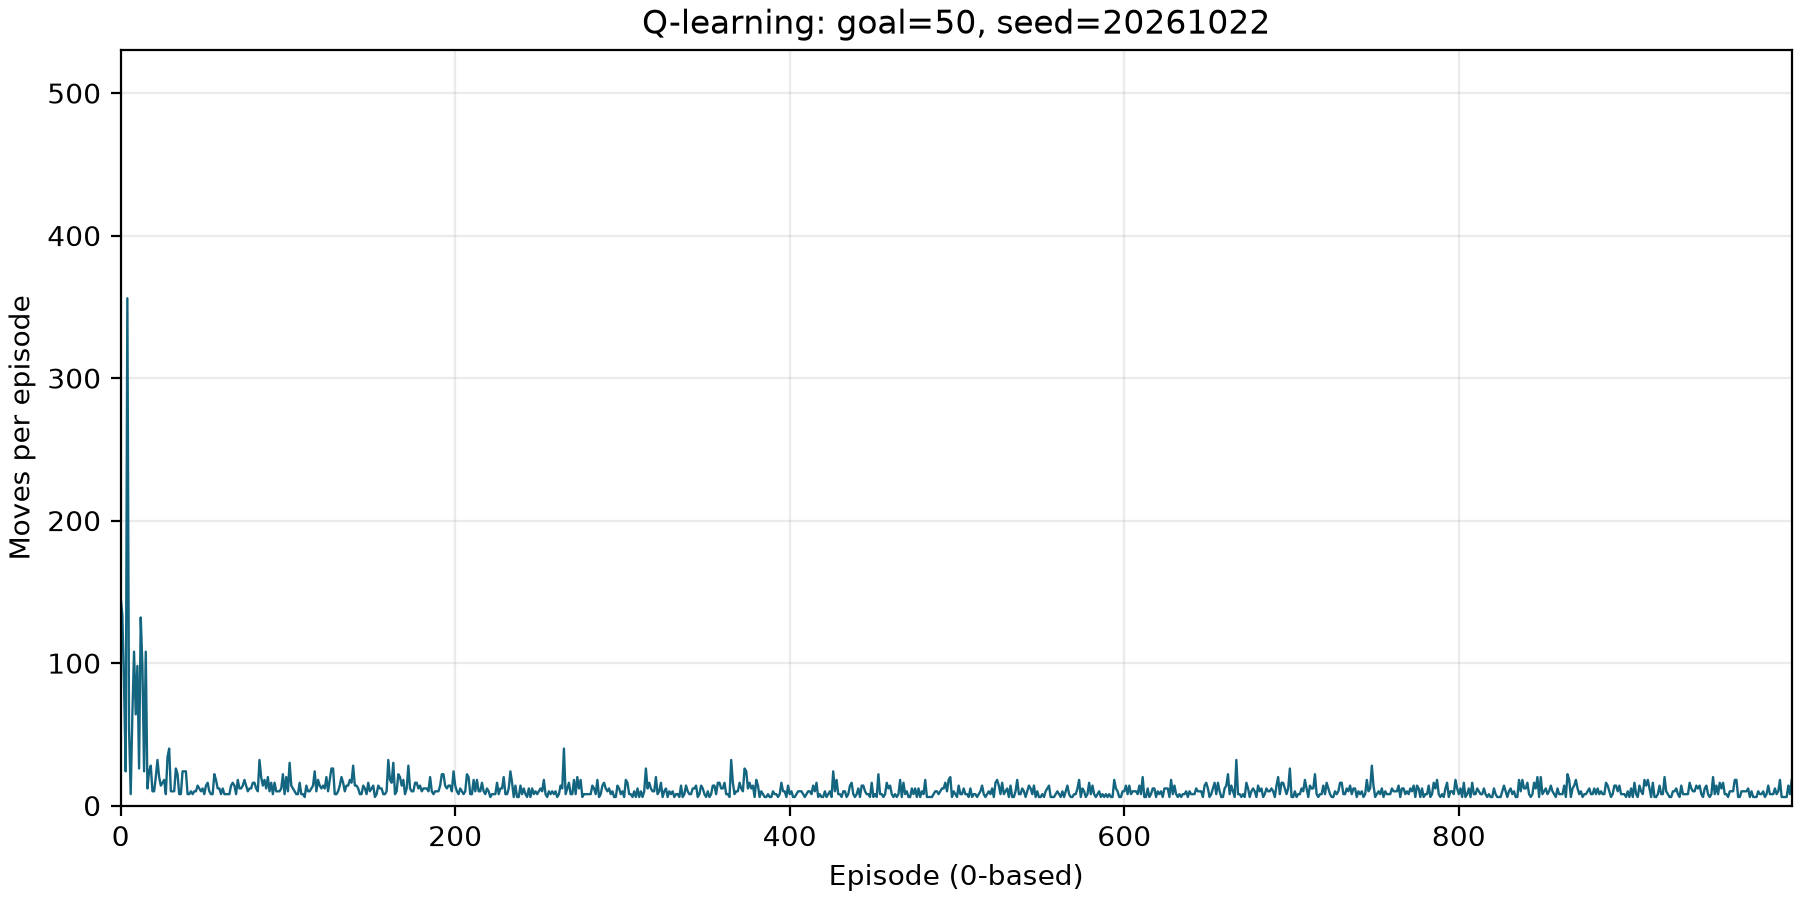
\includegraphics[width=\linewidth]{pc_results/terminal_50/steps.png}
\caption{ゴール50でのステップ数変化}
\label{fig:steps50}
\end{minipage}
\end{figure}

\begin{table}[H]
\centering
\caption{最初と最後の100回の平均移動回数}
\label{tab:steps}
\begin{tabular}{crr}
\hline
ゴール & 最初の100回 & 最後の100回 \\
\hline
54 & 28.48 & 16.06 \\
50 & 27.50 & 10.08 \\
\hline
\end{tabular}
\end{table}

\subsection*{考察}
どちらの条件でも，学習初期に比べて，後半は少ない移動回数でゴールに到達した．
表\ref{tab:steps}より，平均移動回数はゴール54では28.48回から16.06回へ，
ゴール50では27.50回から10.08回へ減少した．
このことから，学習によって遠回りが減り，効率よくゴールに進めるようになったと考えられる．

後半にも移動回数のばらつきが残っている．今回のプログラムでは探索率が0.3のままなので，
学習後も30\%の確率でランダムに移動可能な行動を選ぶ．
この探索が，ときどき遠回りする原因の一つと考えられる．

ゴール50の方が後半の移動回数は少ないが，壁のない今回の盤面では，
開始状態9からの最短距離はゴール54が10回，ゴール50が6回である．
もともとの距離が異なるため，移動回数だけでゴール50の方が学習が速いとは判断できない．

\clearpage
\section*{課題3.3}
PCでの学習終了時に保存した\texttt{q\_table.dat}の数値を確認した．
Qテーブルは64行4列であり，行は状態0から63，列は左から上・下・左・右の行動に対応する．
状態番号は8列の盤面に左上から横方向へ順に付けられている．
表\ref{tab:qvalues}に，Q値が高かった状態・行動対の例を示す．
表示値は小数第3位までとした．

\begin{table}[H]
\centering
\caption{学習終了時のQテーブルから抜粋した状態・行動対}
\label{tab:qvalues}
\begin{tabular}{crcrr}
\hline
ゴール & 状態 & 行動 & 移動先 & Q値 \\
\hline
54 & 53 & 右 & 54 & 100.000 \\
54 & 45 & 下 & 53 & 90.000 \\
54 & 52 & 右 & 53 & 90.000 \\
50 & 42 & 下 & 50 & 100.000 \\
50 & 49 & 右 & 50 & 99.976 \\
50 & 34 & 下 & 42 & 90.000 \\
\hline
\end{tabular}
\end{table}

同じQテーブルから作成したQ値マップを図\ref{fig:qmap54}，図\ref{fig:qmap50}に示す．
各マスでは4方向のQ値の最大値を表示しており，青ほど小さく，赤ほど大きい．
マップには状態番号と最大Q値を併記した．方向ごとの値はQテーブルで確認する必要がある．

\begin{figure}[H]
\centering
\begin{minipage}[t]{0.49\linewidth}
\centering
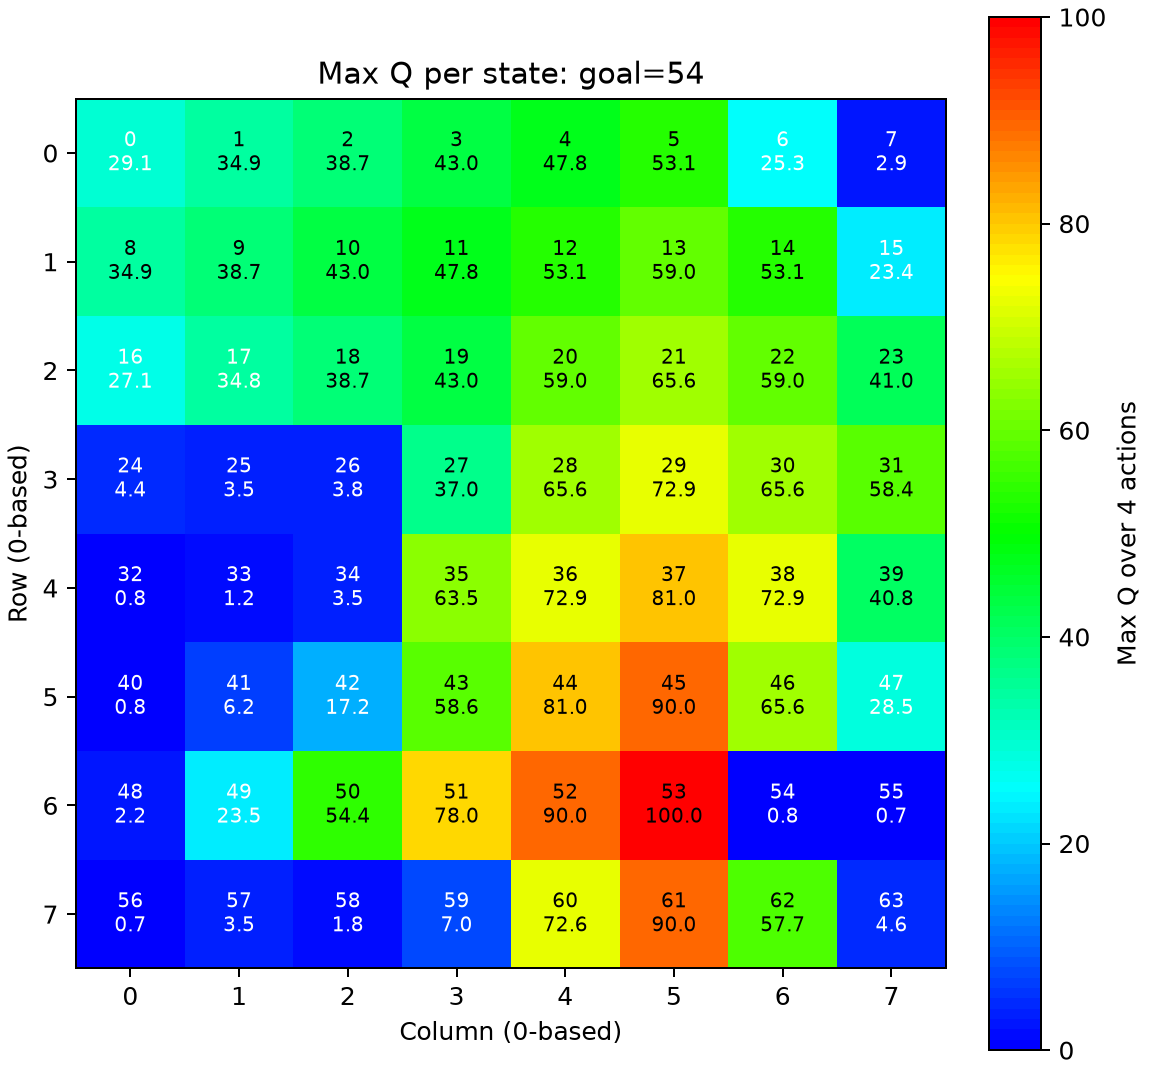
\includegraphics[width=\linewidth]{pc_results/terminal_54/q_map_labeled.png}
\caption{ゴール54でのQ値マップ}
\label{fig:qmap54}
\end{minipage}\hfill
\begin{minipage}[t]{0.49\linewidth}
\centering
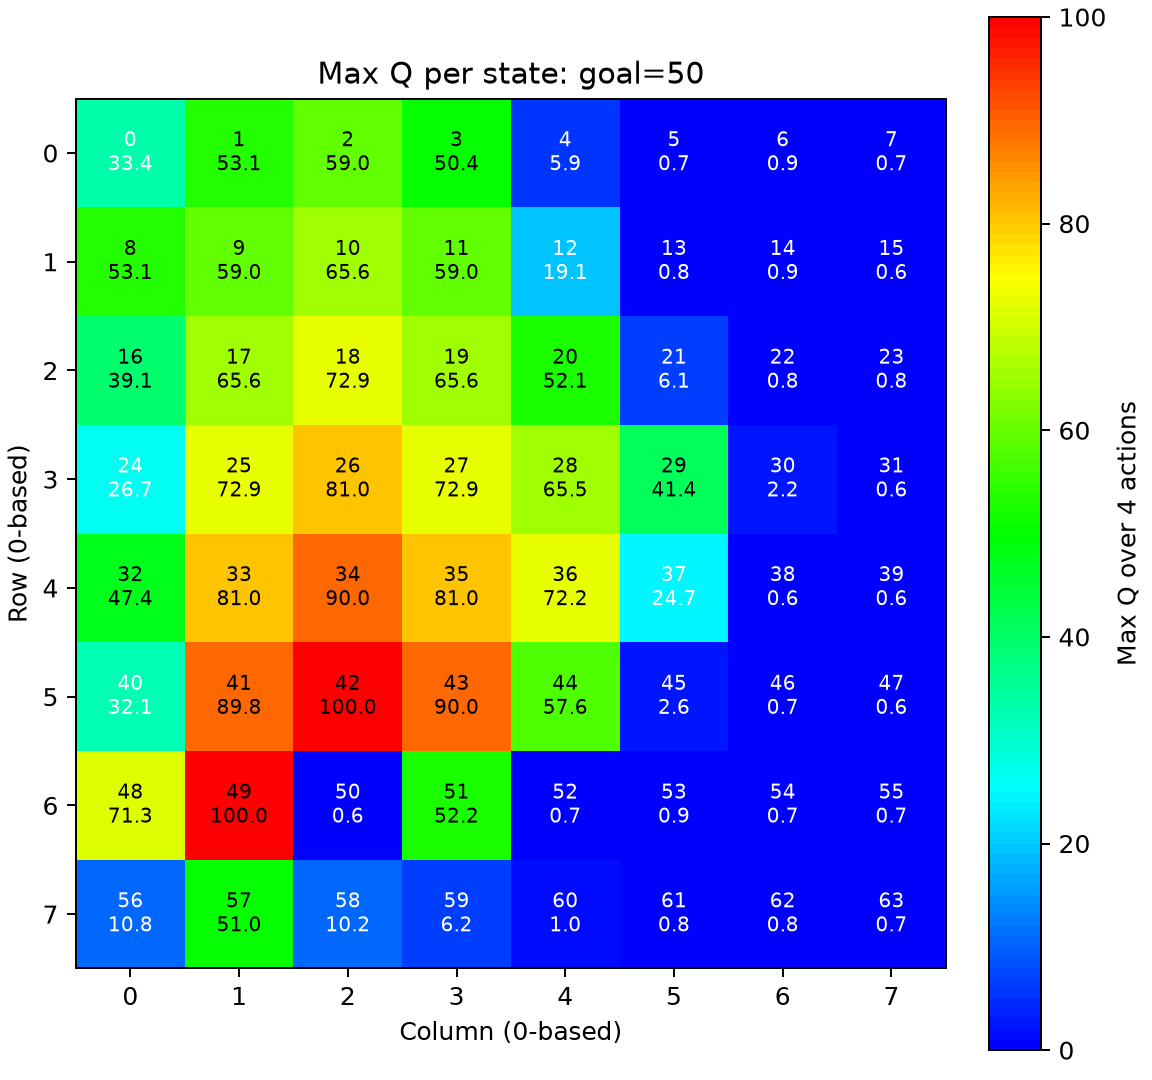
\includegraphics[width=\linewidth]{pc_results/terminal_50/q_map_labeled.png}
\caption{ゴール50でのQ値マップ}
\label{fig:qmap50}
\end{minipage}
\end{figure}

\subsection*{考察}
ゴール54では，左隣の状態53から右へ動く行動のQ値が約100となった．
ゴール50でも，上隣の状態42から下へ動く行動が約100，
左隣の状態49から右へ動く行動が約99.976と高い値になった．
これらはゴールへ直接入る行動である．プログラムではゴール到達時の報酬が100なので，
繰り返し学習することで，これらの行動のQ値が100に近づいたと考えられる．

ゴール54に対して，状態45から下の状態53へ動く行動のQ値は約90だった．
この行動のあとに右へ動けばゴールに到達できる．割引率が0.9なので，
1回先の行動の価値100が$0.9\times100=90$として更新に使われたと考えられる．
したがって，すぐにゴールへ入る行動だけでなく，その先でゴールにつながる行動も高く評価された．

なお，ゴールのマス自体のQ値は小さいままだが，これは到達した時点で試行を終え，
ゴールから先の行動を学習しないためである．ゴールの価値が低いことを意味するわけではない．
また，各行動が選ばれる回数は異なるため，同じ距離の行動でもQ値が完全に一致するとは限らない．
\end{document}
